\chapter{Latent Variable Models}
% Authors: Yash Goel, Urwa Muaz, Soham R Mody
% Lecture date: 4/1/2019

\section{Latent Variable Models: Face Detection}
% Authors: Yash Goel, Urwa Muaz, Soham R Mody
% Lecture date: 4/1/2019

In this section, we take a look at an example of latent variable models in object detection. Consider the following figure. Say we want to train the system for face detection. In this model, \\
X: observed variables (input variables) \\
Y: observed on training set (output variables) \\
Z: never observed (latent variable) \\

We input an image where which may or may not contain a face. The location of the face is also unknown to us so, Z can be considered a latent variable which represents the location of the face. \\

For the sake of the example, let's imagine that this system is composed of a convolutional neural network(CNN) and an energy based model(EBM) on top of it. Using a switch, for values smaller than the threshold T, we decide there is a face and there isn't for others. Because we intend to minimize energy, low values are good and high values are bad for the score. The CNN run overs all the candidate locations of the face and gives a score based on that and the EBM  minimizes the energy with respect to Z and Z is also computed in this process which is the model's best guess about the location of the face. \\

\begin{figure}[t]
\centering
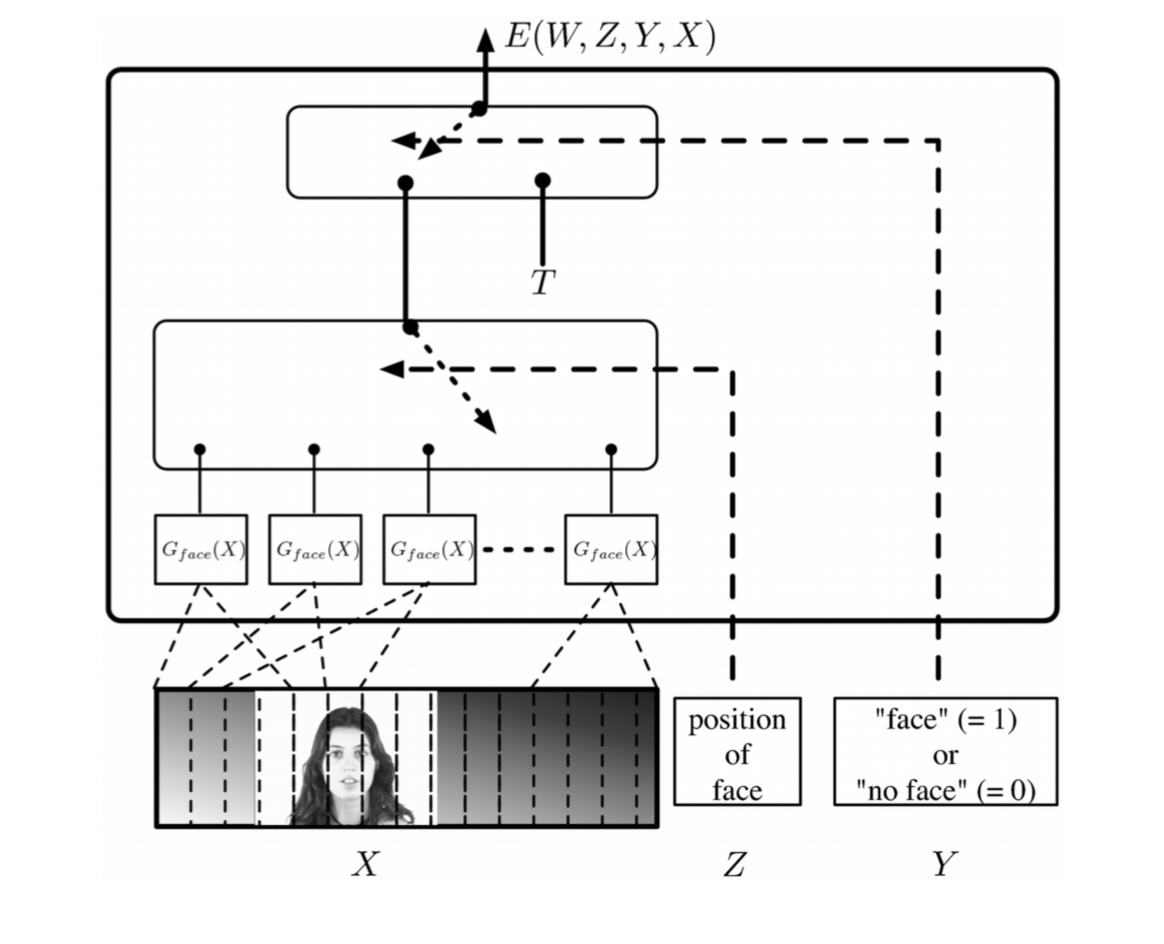
\includegraphics[width=100mm]{lectures/08-b/2.png}
\caption{Training the system for face detection and localisation}
\end{figure}

Our goal is to find the combination of Z and Y that minimises the energy. T This is a good approach for unsupervised learning where we do not know where the face is located in the image. System is only stable when it picks the face and the learning can happen through gradient descent. Marginalization is better because you would not need a switch anymore and it would be a continuous module that you can back propagate through, so learning happens in all scenarios.\\ 

Generally there are two methods involved which are minimizing energy with respect to Z and marginalize energy with respect to Z. The integral for marginalization often requires a lot of approximations.

\section{Latent Variable Models: Integrated training with sequence alignment}
% Authors: Yash Goel, Urwa Muaz, Soham R Mody
% Lecture date: 4/1/2019

Let's look at another example of latent variable models. Say we want to detect a few keywords - Alexa, Hey Google and so on.

These systems consume minimum energy because they run all the time. We can have templates but these templates don't have definite length because the speed of speaking same words is different for different people. Elastic template matching solves this problem and it was previous used in speech recognition systems. You have to minimize the energy for multiple templates and then, you output the template with lowest energy. 

You can do it using dynamic programming by matching up all the features and template features and creating a matrix of distances. After that, you have to traverse through it and choose the path with lowest cost. 

We create a template for each keyword and follow this process:\\
1. Input the sequence\\
2. Extract trainable features to get a sequence of feature vectors\\
3. Then we do elastic matching with the input and the template.\\
4. We do this for every template and then output the template that has the lowest energy.\\

\section{What can latent variables represent?}
% Authors: Yash Goel, Urwa Muaz, Soham R Mody
% Lecture date: 4/1/2019

1. Face recognition: Gender, orientation of the face. \\
2. Object recognition: Pose parameters of the object, lighting conditions.\\
3. Speech Recognition: Segmentation of the sentence into phonemes or phones.\\
4. Handwriting Recognition: segmentation of line into characters.\\
5. Scene Parsing: Segmentation of image into components.\\
6. Parts of speech tagging: Segmentation of sentence into syntactic units.\\

\section{Loss Function}
% Authors: Yash Goel, Urwa Muaz, Soham R Mody
% Lecture date: 4/1/2019

We design a loss function in such a way that the model gives low energy to the inputs that we want and high energy(i.e. cost) to the inputs that we don’t want. We essentially aim to push down on the energy of the correct answer and pull up on the energies of the incorrect answers.

Note: A simple energy loss function faces a "collapse" problem. This is something to pay attention to at the time of training.

\begin{figure}[t]
\centering
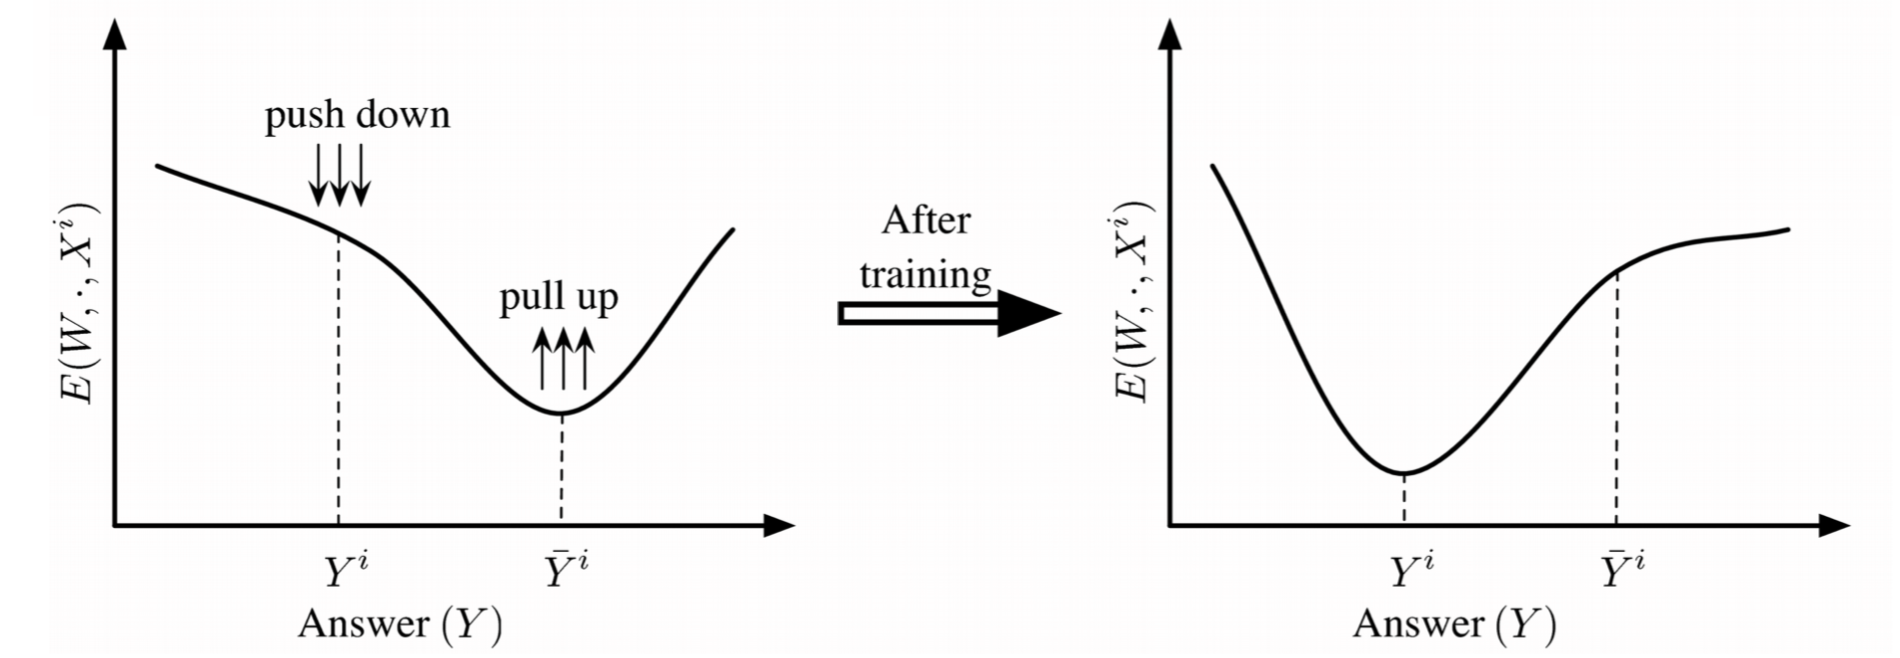
\includegraphics[width=100mm]{lectures/08-b/4.png}
\caption{Loss function before training (left) and after training (right)}
\end{figure}

\subsection{A better loss function: Generalised Margin Losses}
As long as the energy of the incorrect answers is very large as compared to the right answer, the collapse problem won't be there. More specifically, if the energy of the “best wrong answer” is higher than the energy of the correct answer, then the model should work. For e.g. Square Square loss (Figure \ref{fig:sqloss})
\begin{figure}[ht]
\centering
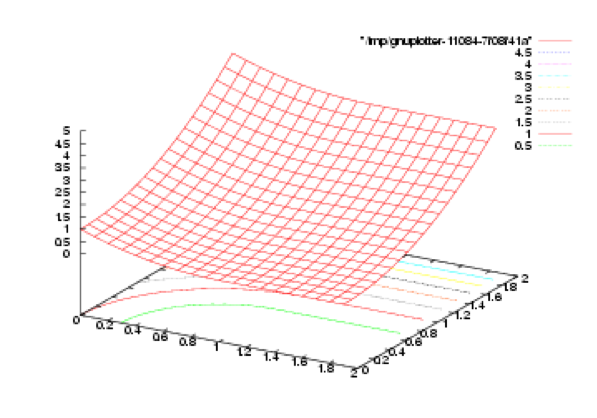
\includegraphics[width=100mm,height=4cm]{lectures/08-b/Square_Square.png}
\caption{Square-Square Loss}
\label{fig:sqloss}
\end{figure}

\section{Approach for EBM models}
% Authors: Yash Goel, Urwa Muaz, Soham R Mody
% Lecture date: 4/1/2019
These are the steps: \\
1. Design an architecture choosing a particular form of energy function E(W,y,X) \\
2. Pick an inference algorithm for Y \\
3. Pick a loss function: In such a way that minimising it with respect to W over a training set will make the inference algorithm find the correct Y for X.\\
4. Pick an optimisation method.

The simplest loss function is the energy itself that the model assigns. 

Consider the example where energy is defined as the L2 norm of difference between outputs of two neural networks. One is fed with X and other with Y. In this scenario, the simplest way for the system to minimize energy is to assign zero weights to both networks and a similar bias term and get energy zero. This is called a collapse.

When calibrated energies at the output are not useful and you are only concerned with making a decision, then you only care about the energy of the correct answer being lower than the rest, the actual values themselves don't matter.

Perceptron loss is a special condition of negative log likelihood.

If an energy function is a linear function of parameters, then we don't have a collapse problem. But if it is non-linear, there are chances of a collapse.
But even then, as long as  the energy of the most offensive incorrect answer is larger than the correct answer, we won't have a collapse. Hinge loss and log loss are examples of such a loss function. 

\begin{figure}[h]
 
\begin{subfigure}{0.5\textwidth}
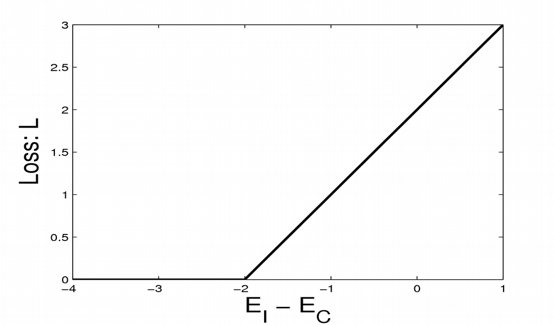
\includegraphics[width=0.9\linewidth, height=5cm]{lectures/08-b/Hinge.png} 
\caption{Hinge Loss}
\label{fig:subim1}
\end{subfigure}
\begin{subfigure}{0.5\textwidth}
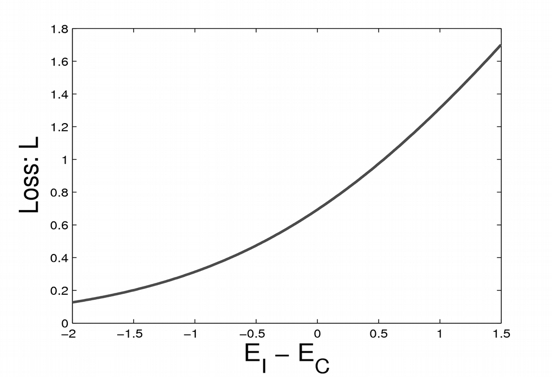
\includegraphics[width=0.9\linewidth, height=5cm]{lectures/08-b/Log_Loss.png}
\caption{Log Loss(Soft-Hinge Loss)}
\label{fig:subim2}
\end{subfigure}
 
\caption{Examples of Generalized Marginal Losses}
\label{fig:image2}
\end{figure}

The table below shows various good and bad loss functions.
\begin{figure}[h]
\centering
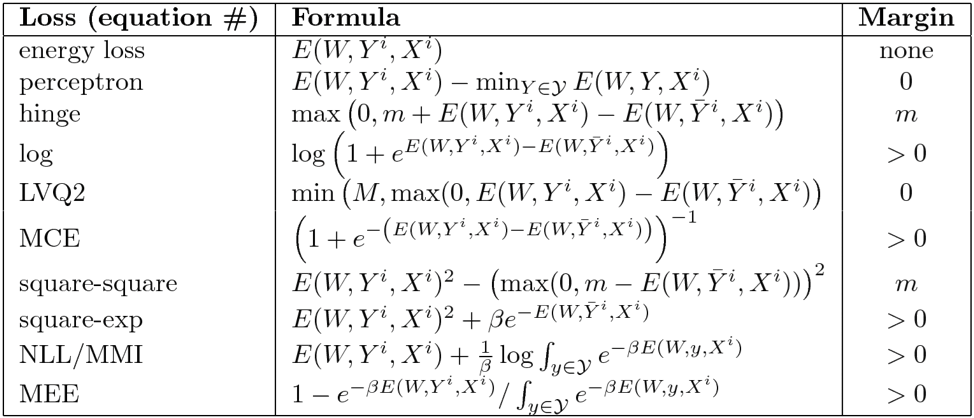
\includegraphics[width=100mm]{lectures/08-b/Good_Bad_Loss.png}
\caption{Good and bad Loss functions}
\end{figure}
 